\documentclass{fmbvecto}

\usepackage[spanish]{babel}

\renewcommand{\title}{Taller 1}
\newcommand{\subject}{Cálculo Vectorial}

\renewcommand{\labelenumii}{\theenumii}
\renewcommand{\theenumii}{\theenumi.\arabic{enumii}.}

\NewDocumentCommand{\itemp}{o}{\item (#1 puntos)}

\begin{document}

Jueves, 13 de junio de 2024

\begin{center}
    \textbf{\LARGE \title} \\
    {\large \subject}
\end{center}


Profesor: Jacinto Eloy Puig Portal, \href{mailto:jpuig@uniandes.edu.co}{jpuig@uniandes.edu.co}. \\
Monitor: Federico Melo Barrero, \href{mailto:f.melo@uniandes.edu.co}{f.melo@uniandes.edu.co}.\\

\textbf{\Large Preámbulo}

Las instrucciones referentes a la entrega del taller están escritas en \href{https://bloqueneon.uniandes.edu.co/d2l/home}{Bloque Neón}.

Como recomendaciones generales, recuerde incluir las unidades siempre que trate con magnitudes físicas, incluso en los pasos y resultados intermedios. No necesita hacer uso de herramientas que le ayuden a hacer matemáticas, ya sean calculadoras, aplicaciones, grandes modelos de lenguaje u otras. Le recomiendo que no lo haga, pues esto irá en detrimento de su aprendizaje.

Se sumarán 0.5 puntos de bonificación a la nota del taller si este satisface las siguientes características: primero, su contenido está ordenado; segundo, todo el texto puede leerse con facilidad; tercero, no contiene errores léxicos, gramaticales ni faltas de ortografía.

\section{Repaso}

Los ejercicios de esta sección pueden ser solucionados sirviéndose únicamente de herramientas conceptuales impartidas en cursos prerrequisitos de Cálculo Vectorial. Si le resulta complicado abordar estos ejercicios, lo espero en la sesión de resolución de dudas, el próximo martes a las 17 horas, en el salón ML 610.

\begin{enumerate}
    \item (Cálculo Diferencial, \(0.\bar{3}\) puntos) Indique un valor \(n \in \mathbb{N} \setminus \{0\}\) tal que \(\frac{3}{4}\) sea un número crítico de la función \(f(x)=x-\sqrt{nx+1}\).

    
    \item (Álgebra Lineal) Sean \(\pi_1, \pi_2, \pi_3 \in \mathbb{R}^3\) los siguientes planos:
    \begin{itemize}
        \item \(\pi_1\) es el plano que pasa por los puntos \((1, 0, 0)\), \((0, 1, 0)\) y \((0, 0, 1)\).
        \item \(\pi_2\) es el plano descrito por \(2x + 2y + 2z = 5\).
        \item \(\pi_3\) es el plano descrito por \(2x + 3y + 4z = 5\).
    \end{itemize}
    \begin{enumerate}
        \itemp[\(0.1\bar{6}\)] Compare \(\pi_1\) y \(\pi_2\): determine si coinciden, son paralelos o se intersecan e indique la distancia entre ellos.
        \itemp[\(0.1\bar{6}\)] Compare de la misma manera a \(\pi_1\) y \(\pi_3\).
        \itemp[\(0.\bar{3}\)] Tras comparar \(\pi_1\) con \(\pi_2\) y \(\pi_1\) con \(\pi_3\), habrá notado que solo un par se intersecan. Determine si la recta en la que intersecan se interseca con \(\ell(t) = (1+t, 2-t, 2t)\).
    \end{enumerate}
\end{enumerate}

\section{Funciones}
    \begin{enumerate}
        \setcounter{enumi}{2}
        \itemp[\(0.08\bar{3}\)] A cada una de las siguientes funciones, atribúyale todas las categorías que le correspondan, entre: univariada, multivariada, escalar, vectorial, campo vectorial y real.
        \begin{align*}
            &f(x, y) = -2x^2 - 3y^2. &&
    		g\colon\begin{pmatrix}
                x_1\\x_2\\x_3\\x_4\\x_5\end{pmatrix}\mapsto\cos(x_1+x_3)+\sin(x_2+x_4)+\mathrm{e}^{x_5}.\\&
                    \bvec{F}(x) = \begin{pmatrix}
                        x^{x} \\ (1+x) / x^5 \\ \tanh x \\ x
                    \end{pmatrix}. &&
            \bvec{G}\colon\begin{pmatrix}
            x\\y\\z
            \end{pmatrix}\mapsto\begin{pmatrix}
            \ln(x+y) \\ x^2 \\ \tan(x-y) \\y^2 \\ x^2+y^2 \\ \operatorname{arccsc}(y)
            \end{pmatrix}.
        \end{align*}


        \item Para cada una de las funciones del punto anterior cuya gráfica sea un subconjunto de \(\mathbb{R}^3\):
        %que sea posible dibujar en papel:
        \begin{enumerate}
            \itemp[\(0.08\bar{3}\)] Grafique por lo menos un conjunto de nivel. Graficar varios puede resultarle útil.
            \itemp[\(0.08\bar{3}\)] Para cada conjunto de nivel graficado, si su gráfica forma una figura con nombre, escriba el nombre.
            \itemp[\(0.08\bar{3}\)] Dibuje la gráfica de la función.
        \end{enumerate} 
    \end{enumerate}


\section{Límites}

Demuestre la existencia o inexistencia de los siguientes límites.

\begin{enumerate}
    \setcounter{enumi}{4}
    \itemp[\(0.\bar{3}\)] \(\displaystyle \lim_{(x, y) \to (1, 0)} \frac{(x-1)^2+2(x-1)y}{(x-1)y}\).
    \itemp[\(0.\bar{3}\)] \(\displaystyle  \lim_{(x, y) \to (0, 0)} \frac{x^3+y^3}{xy}.\)
\end{enumerate}

\section{Diferenciación}

\begin{enumerate}
    \setcounter{enumi}{6}
    \itemp[\(0.\bar{3}\)] Demuestre o refute que \(f(x, y) = \cos(xy) +x\cos(y)\) es diferenciable para cualesquiera \(x, y \in \mathbb{R}\).
    \itemp[\(0.\bar{3}\)] Halle el plano que es tangente a la gráfica de \(g(x, y) = x^2+y^4+e^{xy}\) en el punto \((1, 0, 2)\). Elija y enuncie un punto \((x, y) \in \mathbb{R}^2\) en el cual no haya un extremo de \(g\) y explique su elección.
    \itemp[\(0.\bar{3}\)] Pedro es un extraterrestre de uno de los satélites de Saturno, Titán. Pedro precisa de altas concentraciones de nitrógeno para su supervivencia. La concentración percibida de nitrógeno con respecto a la ubicación en Titán está modelada por la función \(N(x, y, z) = x^2+y^4+2z^2\), donde \(x\), \(y\) y \(z\) están medidas en decámetros y \(N(x, y, z)\) está medida en \(\mathrm{mg} \, \mathrm{L}^{-1}\). 
    
    Pedro se está empezando a sentir sofocado por carencia de nitrógeno. Decide desplazarse en línea recta en la dirección en la que la concentración de nitrógeno incrementa más rápidamente. Si él sabe que está ubicado en el punto \((1, 1, 1)\), ¿en qué dirección debe avanzar en aras de convalecerse? Al desplazarse en esa dirección, ¿cuál es la tasa de cambio de la concentración de nitrógeno?
    \begin{figure}[H]
        \centering
        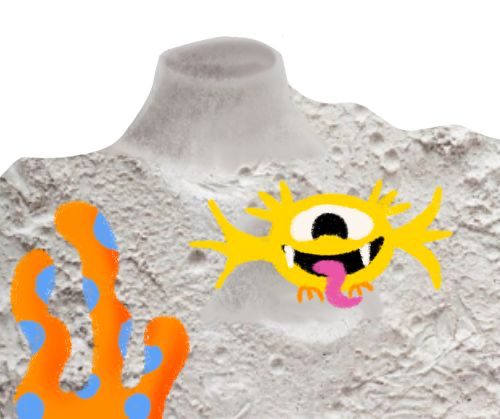
\includegraphics[width=0.3\textwidth]{marciano.png}
        \caption{Pedro.}
    \end{figure}
\end{enumerate}

\section{Optimización}

\begin{enumerate}
    \setcounter{enumi}{9}
    \itemp[\(0.\bar{3}\)]  Enuncie dos métodos distintos para hallar los extremos locales de una función restringida a un compacto. ¿Existen circunstancias bajo las cuáles un método es preferible al otro? Si sí, provea un ejemplo; de lo contrario, explique su raciocinio.
    
    \itemp[\(0.\bar{3}\)]  Dada la función \(f(x,y)=x^2+y^2-2y\) definida en el disco \(x^2+y^2\leq 4\), indique cuáles son los extremos de la función en ese disco. 
    
    \itemp[\(0.\bar{3}\)]  De todos los puntos contenidos en \(y\sqrt{x} = \sqrt{2}\) indique cuál es el más cercano al origen.

    
    \itemp[\(0.\bar{3}\)] Suponga que cuenta con \(12 \, \mathrm{cm}^2 \) de cartón que usará como material para las paredes y el piso de una caja rectangular sin tapa. Desprecie la forma en la que unirá las paredes entre sí y no contemple tampoco el grosor del cartón.
    \begin{itemize}
        \item Dibuje una caja que podría armar con ese material sin desperdiciar material. Indique las dimensiones de la caja en el dibujo.
        \item Dibuje la caja que se puede armar con ese material que maximice el volumen de líquido que puede contener. Indique las dimensiones de esta caja en el dibujo. Explique por qué está seguro de que, bajo las mismas condiciones, no se puede construir otra caja de mayor volumen.
    \end{itemize}
    \begin{figure}[H]
        \centering
        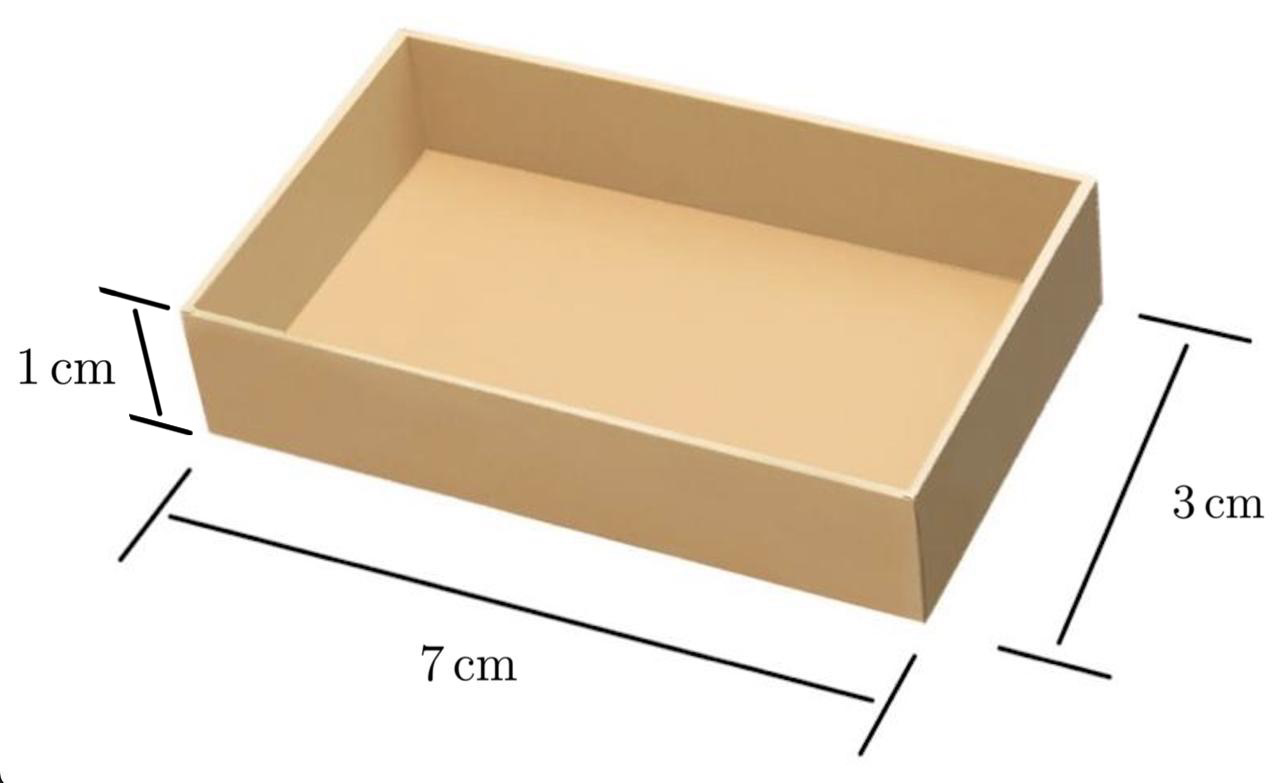
\includegraphics[width=0.5\textwidth]{caja.png}
        \caption{Dibujo de una caja rectangular sin tapa con sus dimensiones indicadas, construida con \(41 \, \mathrm{cm}^2 \) de cartón. Note que el dibujo no está a escala; el suyo tampoco debe estarlo.}
    \end{figure}
        
        
\end{enumerate}

\section{Funciones con valores vectoriales}

\begin{enumerate}
    \setcounter{enumi}{13}
    \item Sea \(\sigma\colon [0,2] \to \mathbb{R}^{3}\) la trayectoria dada por \(\sigma (t) = \left(1,t,\frac{t^3}{3}\right)\) donde las unidades de distancia son los metros y \(t\) está medida en segundos.
    \begin{enumerate}
        \itemp[\(0.\bar{1}\)] Indique la velocidad.
        \itemp[\(0.\bar{1}\)] Indique la rapidez.
         \itemp[\(0.\bar{1}\)] Indique la longitud de la trayectoria.
    \end{enumerate}
    \itemp[\(0.\bar{3}\)] Sea \(U \subseteq \mathbb{R}^{m}\) un conjunto abierto y sean \(\bvec{F},\bvec{G}\colon U\to \mathbb{R}^{n}\) campos vectoriales. Demuestre o refute la siguiente propiedad:
\[\div (\bvec{F} \times \bvec{G}) = \nabla \cdot (\bvec{F} \times \bvec{G}) = \bvec{G}\cdot \rot\bvec{F} - \bvec{F}\cdot \rot \bvec{G}.\]
\end{enumerate}


\end{document}
